\documentclass[
	% -- opções da classe memoir --
	12pt,				% tamanho da fonte
	openright,			% capítulos começam em pág ímpar (insere página vazia caso preciso)
	oneside,			% para impressão em frente e verso. Oposto a oneside
	a4paper,			% tamanho do papel.
	% -- opções da classe abntex2 --
	english,			% idioma adicional para hifenização
	brazil				% o último idioma é o principal do documento
	]{abntex2}


% --- PACOTES BÁSICOS ---
\usepackage{mathptmx}			% Usa a fonte Times New Roman
\usepackage[T1]{fontenc}		% Selecao de codigos de fonte.
\usepackage[utf8]{inputenc}		% Codificacao do documento (acentos)
\usepackage{lastpage}			% Usado pela Ficha catalográfrica
\usepackage{indentfirst}		% Indenta o primeiro parágrafo de cada seção.
\usepackage{graphicx}			% Inclusão de gráficos
\usepackage{subcaption}			% Inclusão de gráficos lado a lado
\usepackage{tabularx,ragged2e}	% Para inserir tabelas
\usepackage{multirow}			% Para mesclar células
\usepackage[dvipsnames,table,xcdraw]{xcolor}
\usepackage{fancyvrb}			% Permite adicionar arquivos de texto
\usepackage[portuguese, ruled, linesnumbered]{algorithm2e} % Uso de algoritmos
\usepackage{amsfonts}			% Permite usar notação de conjuntos
\usepackage{amsmath}			% Permite citar equações
\usepackage{amsthm}				% Permite criar teoremas e experimentos
\usepackage[font={bf, small}, labelsep=endash, labelfont=bf]{caption}
\usepackage{cancel}				% Permite fazer expressão tendendo a zero
\usepackage{epstopdf}			% Converte eps para pdf
\usepackage[final]{pdfpages}
\usepackage{hyphenat}
\usepackage{enumitem}
\usepackage{lipsum}
\usepackage{modelo-ufpa/ufpa}
\usepackage{booktabs} % no preâmbulo
\usepackage{float}

% --- AJUSTE PARA NBR 10520:2023 ---
% Adicionada a opção 'abnt-cite-style=authoryear-lowcase' para que as citações
% (e.g., FULANO, 2023) apareçam como (Fulano, 2023), conforme a nova norma.
\usepackage[alf, abnt-emphasize=bf, abnt-show-options=doi=on,url=on, abnt-cite-style=authoryear-lowcase]{abntex2cite}



% --- CONFIGURAÇÕES DE LAYOUT E TÍTULOS ---

% Altera a fonte das seções (padrão abntex2) para não ser mais negrito
\renewcommand{\ABNTEXchapterfontsize}{\normalsize}
\renewcommand{\ABNTEXsectionfontsize}{\normalsize}
\renewcommand{\ABNTEXsubsectionfontsize}{\normalsize}
\renewcommand{\ABNTEXsectionfont}{}
\renewcommand{\ABNTEXsubsectionfont}{}

% Seções
\renewcommand{\cftsectionindent}{2.5em}
\renewcommand{\cftsectionnumwidth}{3.5em}

% Subseções
\renewcommand{\cftsubsectionindent}{5em}
\renewcommand{\cftsubsectionnumwidth}{4.5em}


% --- ESTILO DE PÁGINA ---
\makepagestyle{ultima}
\makeoddhead{ultima}{}{}{\thepage}
\makeevenhead{ultima}{}{}{\thepage}
\makeheadrule{ultima}{0pt}{0pt}
\makefootrule{ultima}{0pt}{0pt}

% --- CAMINHO DAS IMAGENS ---
\graphicspath{{imagens/}}

% --- AMBIENTE DE EXPERIMENTOS ---
\theoremstyle{definition}
\newtheorem{experimento}{Experimento}[section]
\newcommand{\experimentoautorefname}{Experimento}

% --- INFORMAÇÕES DA CAPA E FOLHA DE ROSTO (COMANDOS DO PACOTE UFPA) ---
\universidade{Centro Universitário Serra dos Órgãos \- UNIFESO}
\instituto{Direção Acadêmica de Ciências Humanas e Tecnológicas \- DACHT}
\curso{Curso de Bacharelado em Ciência da Computação}
\titulo{Orbitar: Uma plataforma web para o reaproveitamento de eletrônicos e promoção da economia circular}
\autor{Letícia Lindberght da Costa}
\local{Teresópolis}
\data{2025}
\orientador{Prof. Nome do Orientador}
\tipotrabalho{Monografia}
\preambulo{Trabalho de Conclusão de Curso apresentado ao Centro Universitário Serra dos Órgãos como requisito obrigatório para obtenção do título de Bacharel em Ciência da Computação.}
\sobrenome{Lindberght}
\nome{Letícia}
\palavraschave{Palavra-chave1, Palavra-chave2, Palavra-chave3}

\datadadefesa{Data da Defesa: 28 de Novembro de 2025}
\faculdadedoorientador{Faculdade do Orientador}
\titulacaodoorientador{MSc}
\faculdadedocoorientador{Faculdade do Coorientador}
\titulacaodocoorientador{DSc}
\primeiromembrodabanca{Nome do Primeiro Membro da Banca}
\titulacaodoprimeiromembro{DSc}
\faculdadedoprimeiromembrodabanca{Faculdade do Primeiro Membro da Banca}
\segundomembrodabanca{Nome do Segundo Membro da Banca}
\titulacaodosegundomembro{DSc}
\faculdadedosegundomembrodabanca{Faculdade do Segundo Membro da Banca}

% --- CONFIGURAÇÕES DE APARÊNCIA DO PDF ---
\definecolor{blue}{RGB}{41,5,195}
\hypersetup{
    pdftitle={\texorpdfstring{\imprimirtitulo}{Orbitar \- Plataforma Web de Reaproveitamento de Eletrônicos}}, 
    pdfauthor={\texorpdfstring{\imprimirautor}{Letícia Lindberght da Costa}},
    pdfsubject={\texorpdfstring{\imprimirpreambulo}{Trabalho de Conclusão de Curso}},
    pdfkeywords={\texorpdfstring{\imprimirpalavraschave}{Palavra-chave1, Palavra-chave2, Palavra-chave3}},
    colorlinks=true,
    linkcolor=black,
    citecolor=black,
    filecolor=magenta,
    urlcolor=black,
    bookmarksdepth=4,
    breaklinks=true
}

% --- ESPAÇAMENTOS ---
\setlength{\parindent}{1.5cm}
\setlength{\parskip}{0.2cm}

% --- COMPILA O ÍNDICE REMISSIVO ---
\makeindex

% ----
% Início do documento
% ----
\begin{document}

% Seleciona o idioma
\selectlanguage{brazil}

% Retira espaço extra obsoleto entre as frases.
\frenchspacing 

% ----------------------------------------------------------
% ELEMENTOS PRÉ-TEXTUAIS
% ----------------------------------------------------------
\pretextual{}

% --- Capa ---
\imprimircapa{}

% --- Folha de rosto ---
\imprimirfolhaderosto{}

% --- Ficha Catalográfica ---
% \begin{fichacatalografica}
%    \includepdf{fichacatalografica.pdf}
% \end{fichacatalografica}
\newpage

% --- Folha de Aprovação ---
\begin{folhadeaprovacao}
\imprimirfolhadeaprovacao{}
\end{folhadeaprovacao}

% --- Dedicatória ---
\begin{dedicatoria}
    \vspace*{\fill}
    \flushright{}
    \textit{Este trabalho é dedicado às crianças adultas que,
	quando pequenas, sonharam em se tornar cientistas.
	\- Lauro César em abnTeX2}
\end{dedicatoria}

% --- Agradecimentos ---
\begin{agradecimentos}
Escreva aqui os seus agradecimentos da maneira que melhor lhe convêm.
\end{agradecimentos}

% --- Epígrafe ---
\begin{epigrafe}
    \vspace*{\fill}
	\begin{flushright}
		\textit{``Que todos os nossos esforços estejam sempre focados no desafio à impossibilidade.\\ Todas as grandes conquistas humanas vieram daquilo que parecia impossível''.\\
		(Charles Chaplin)}
	\end{flushright}
\end{epigrafe}

% --- Resumos ---
\setlength{\absparsep}{18pt}
\begin{resumo}
Escreva aqui o resumo do seu trabalho.

\textbf{Palavras-chave}: \imprimirpalavraschave{}
\end{resumo}

\begin{resumo}[Abstract]
 \begin{otherlanguage*}{english}
   Escreva aqui o seu abstract (Resumo em inglês)
   \vspace{\onelineskip}
   \noindent 
   \textbf{Keywords}: Keywords1. Keywords2. Keywords3.
 \end{otherlanguage*}
\end{resumo}

% --- Listas ---
\pdfbookmark[0]{\listfigurename}{lof}
\listoffigures*
\cleardoublepage{}

\pdfbookmark[0]{\listofquadrosname}{loq}
\listofquadros*
\cleardoublepage{}

\pdfbookmark[0]{\listtablename}{lot}
\listoftables*
\cleardoublepage{}

\pdfbookmark[0]{\listalgorithmcfname}{loa}
\imprimirlistadealgoritmos{}
\cleardoublepage{}

\begin{siglas}
  \item[ABNT] Associação Brasileira de Normas Técnicas
  \item[API] Application Programming Interface (Interface de Programação de Aplicações)
  \item[BFRs] Brominated Flame Retardants (Retardantes de Chama Bromados)
  \item[CGI.br] Comitê Gestor da Internet no Brasil
  \item[OCDE] Organização para a Cooperação e Desenvolvimento Econômico
  \item[REEE] Resíduos de Equipamentos Elétricos e Eletrônicos
  \item[REST] Representational State Transfer (Transferência de Estado Representacional)
  \item[SGBD] Sistema de Gerenciamento de Banco de Dados
  \item[TI] Tecnologia da Informação
  \item[TIC] Tecnologias da Informação e Comunicação
\end{siglas}
% --- Sumário ---
\pdfbookmark[0]{\contentsname}{toc}
\tableofcontents*
\cleardoublepage{}

% ----------------------------------------------------------
% ELEMENTOS TEXTUAIS
% ----------------------------------------------------------
\textual{}
\pagestyle{simple}

% Capítulos
% =================================================================================
% CAPÍTULO 1 - INTRODUÇÃO
% =================================================================================
\chapter[Introdução]{INTRODUÇÃO}

As Tecnologias da Informação e Comunicação (TIC) são pilares da sociedade contemporânea, catalisando o progresso social e econômico. Contudo, o modelo de produção que as sustenta gerou um problema crítico: o descarte precoce de equipamentos eletrônicos, que acelera a formação do lixo eletrônico (e-waste). Este fenômeno é o resultado direto de um sistema caracterizado pela obsolescência programada e por padrões de consumo que normalizam a substituição de dispositivos ainda em plenas condições de uso.

A consequência direta desse descarte acelerado é documentada por múltiplas fontes globais. O relatório \textit{Global E-waste Monitor 2024} revela que a geração de lixo eletrônico atingiu um recorde histórico, crescendo a uma taxa cinco vezes superior à da reciclagem documentada~\cite{forti2024}. Para além do volume, a periculosidade desses resíduos é um fator crítico, dada a presença de substâncias tóxicas como chumbo e mercúrio, que representam uma séria ameaça à saúde e aos ecossistemas quando manuseados incorretamente~\cite{perkins2014}.

Este cenário reflete um desafio sistêmico maior. Segundo a Organização para a Cooperação e Desenvolvimento Econômico (OCDE), os atuais padrões de extração e uso de materiais são insustentáveis~\cite{oecd2019}. Portanto, intervir no ciclo do descarte precoce é uma dupla necessidade: por um lado, mitigar a contaminação ambiental e, por outro, romper com um modelo econômico extrativista e desperdiçador. A solução mais eficaz, alinhada aos princípios da economia circular, é atuar no momento da decisão do descarte, antes que um equipamento funcional se torne resíduo.

Neste contexto, a reutilização emerge como a estratégia prioritária. É a partir desta premissa que este trabalho se desenvolve, propondo uma solução tecnológica para transformar um problema gerado pela própria tecnologia. O objetivo é criar uma ferramenta que ofereça um destino útil para eletrônicos subutilizados, transformando o que seria um desperdício de potencial em um ativo social e promovendo, como valioso benefício secundário, a inclusão digital.

\section[Motivação]{Motivação}

A motivação central deste projeto nasce da constatação de uma grande lacuna no ciclo de vida dos eletrônicos: a ausência de um caminho simples e confiável para o reaproveitamento de equipamentos funcionais que são substituídos. Para um cidadão ou empresa, o processo para dar um destino sustentável a um dispositivo usado é frequentemente opaco e inconveniente. Estudos sobre a gestão de resíduos no Brasil apontam que a falta de canais acessíveis e a desinformação são barreiras significativas~\cite{GreenEletron2022}. Na ausência de uma alternativa clara para a doação, a opção mais fácil se torna o armazenamento indefinido ou, pior, o descarte, que transforma um ativo potencial em lixo eletrônico~\cite{forti2024}.

Por outro lado, existe uma demanda latente e socialmente urgente por esses mesmos dispositivos. A exclusão digital no Brasil é um reflexo direto da desigualdade socioeconômica, onde o alto custo de equipamentos novos é um obstáculo para milhões de famílias. A pesquisa TIC Domicílios evidencia essa barreira, mostrando que a posse de um computador — ferramenta essencial para a educação — ainda é significativamente menor nas classes D e E~\cite{cgi2024}. Essa realidade cria um paradoxo: de um lado, dispositivos plenamente funcionais são descartados prematuramente; de outro, uma vasta parcela da população carece de acesso a essa mesma tecnologia.

Nesse contexto, a tecnologia pode, ironicamente, resolver um problema que ela mesma ajudou a criar. A proposta é desenvolver a \textbf{Orbitar}, uma aplicação web que atue como uma ponte, conectando quem deseja repassar um eletrônico funcional com quem pode dar a ele uma nova vida, tornando o processo de reutilização simples, seguro e geograficamente acessível.

\section[Justificativa]{Justificativa}

A relevância deste trabalho se justifica pela necessidade urgente de se contrapor ao descarte precoce e ao modelo de consumo linear. A importância de intervir nesse ciclo reside em seu duplo impacto negativo: primeiro, os riscos ambientais e de saúde pública causados pelos componentes tóxicos, caso o descarte seja inadequado~\cite{perkins2014}; segundo, o esgotamento de recursos naturais, desperdiçados quando equipamentos úteis são descartados.

A plataforma \textbf{Orbitar} ataca diretamente essa questão, alinhando-se aos princípios da economia circular ao promover a reutilização~\cite{ellen2023}. Ao estender a vida útil de um produto que seria descartado precocemente, evitam-se os impactos da produção de um novo e do descarte de um antigo. Como um benefício social derivado, a plataforma aborda a persistente desigualdade digital no Brasil. Dados da pesquisa TIC Domicílios~\cite{cgi2024} mostram que a posse de um computador ainda é um forte indicador de oportunidade. Portanto, a proposta se justifica por criar um mecanismo que ataca a raiz do desperdício e, como consequência, transforma um passivo ambiental em um ativo para a inclusão social.

\section[Objetivos]{Objetivos}

Diante do cenário exposto, os objetivos deste trabalho são definidos a seguir.

\subsection[Objetivo Geral]{Objetivo Geral}

Desenvolver a Orbitar, uma aplicação web focada em promover a economia circular e a sustentabilidade, que conecte doadores e receptores de produtos eletrônicos de forma organizada, segura e localizada, a fim de mitigar o descarte precoce de e-waste e estender a vida útil da tecnologia.

\subsection[Objetivos Específicos]{Objetivos Específicos}

Para alcançar o objetivo geral, os seguintes objetivos específicos foram definidos:

\begin{enumerate}[label={\alph*}]
    \item Desenvolver um sistema de cadastro e autenticação de usuários (doadores e receptores) para garantir um ambiente seguro para as transações;
    \item Implementar a funcionalidade de registro de produtos eletrônicos para doação, incluindo campos para descrição, categoria, estado de conservação e localização;
    \item Construir uma interface de busca e filtragem de eletrônicos baseada em geolocalização, permitindo que receptores encontrem doações próximas;
    \item Modelar e implementar o fluxo completo de doação, incluindo a reserva de um item por um receptor, a comunicação entre as partes e a confirmação de entrega;
    \item Integrar um sistema de avaliação mútua entre usuários para construir uma relação de confiança na comunidade da plataforma.
\end{enumerate}
\section[Organização do Trabalho]{Organização do Trabalho}

O restante deste trabalho está organizado da seguinte forma: o Capítulo 2 apresenta a fundamentação teórica, abordando os conceitos de e-waste como consequência do descarte precoce, a economia circular e as tecnologias que servem de base para o projeto. O Capítulo 3 apresenta a revisão da literatura, analisando soluções existentes e identificando as lacunas que justificam a proposta. O Capítulo 4 descreve detalhadamente a metodologia empregada, incluindo a arquitetura do sistema, o modelo de dados e as ferramentas utilizadas no desenvolvimento. No Capítulo 5, são apresentados os resultados, com a demonstração das funcionalidades da plataforma. Finalmente, o Capítulo 6 traz as considerações finais, discutindo as conclusões do estudo, as limitações encontradas e as sugestões para trabalhos futuros.

% =================================================================================
% CAPÍTULO 2 - FUNDAMENTAÇÃO TEÓRICA
% =================================================================================
% =================================================================================
% CAPÍTULO 2 - FUNDAMENTAÇÃO TEÓRICA (COM POSICIONAMENTO CORRIGIDO)
% =================================================================================
\chapter[Fundamentação Teórica]{FUNDAMENTAÇÃO TEÓRICA}

Esta seção tem o objetivo de fundamentar os conceitos que sustentam este trabalho. Inicia-se pela contextualização do modelo de produção linear e suas consequências, aprofunda-se no problema do descarte precoce de eletrônicos e, por fim, apresenta-se a economia circular como o paradigma de solução que orienta o desenvolvimento da plataforma \textbf{Orbitar}.

\section{A Economia Linear e a Cultura do Descarte}

O modelo econômico predominante desde a Revolução Industrial é a economia linear, cujo fluxo de materiais segue uma lógica unidirecional: extrair, produzir, usar e descartar (Figura~\ref{fig:economia-linear}). Este sistema trata os recursos naturais como se fossem inesgotáveis e não atribui valor a um produto após seu primeiro ciclo de vida, gerando um volume massivo de resíduos.

\begin{figure}[H] % <-- NOTA: [H] força a figura a aparecer aqui.
    \centering
    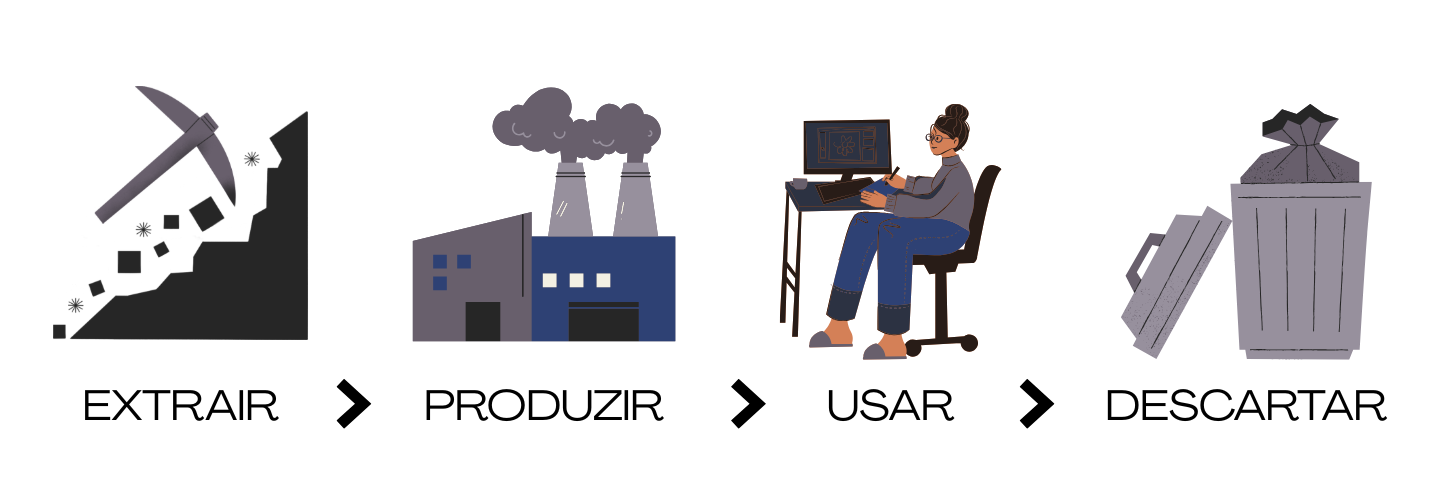
\includegraphics[width=0.9\textwidth]{imagens/economia_linear.png}
    \caption{Fluxo do Modelo de Economia Linear.}
    \label{fig:economia-linear}
    \legend{Fonte: Adaptado de Ellen MacArthur Foundation (2013).}
\end{figure}

Associada a esse modelo, a obsolescência programada emerge como uma estratégia deliberada para encurtar a vida útil dos produtos, seja por limitações de hardware, incompatibilidade de software ou dificuldade de reparo. Essa prática, combinada com o marketing que incentiva a troca constante por novos modelos, acelera o ciclo de consumo e é a principal causa do descarte precoce de equipamentos eletrônicos, muitas vezes ainda em perfeito estado de funcionamento~\cite{Forti2020}.

\section{O Problema do Descarte Precoce e suas Consequências}

O descarte precoce de eletrônicos é o ato de se desfazer de um dispositivo funcional, transformando-o prematuramente em lixo eletrônico (e-waste). Essa prática agrava um problema já crítico, cujas consequências são de ordem ambiental e social.

\subsection{Composição e Impactos do E-waste}

O lixo eletrônico possui uma composição complexa. Embora contenha materiais valiosos que o caracterizam como "minério urbano"~\cite{Robinson2009}, sua maior ameaça reside nos componentes tóxicos, como chumbo, mercúrio e cádmio~\cite{Widmer2005}. O manejo inadequado desses resíduos contamina o solo e a água, além de expor populações a riscos de saúde, como danos neurológicos e doenças respiratórias~\cite{perkins2014b, Heacock2016}. O descarte precoce intensifica esses impactos ao aumentar desnecessariamente o volume de resíduos perigosos gerados.

\section{A Economia Circular como Paradigma de Solução}

Em contraposição ao modelo linear, a economia circular propõe um sistema regenerativo, onde o valor dos produtos e materiais é mantido em circulação pelo maior tempo possível. Seus princípios são: eliminar resíduos, manter produtos em uso e regenerar sistemas naturais~\cite{EMF2013}.

Para operacionalizar este conceito, utiliza-se a hierarquia de estratégias conhecida como os "5 Rs" (Figura~\ref{fig:hierarquia-5Rs}), onde a Reutilização se destaca como uma das ações de maior valor, sendo superior à reciclagem. Reutilizar um produto conserva toda a energia, trabalho e materiais embutidos em sua fabricação, enquanto a reciclagem recupera apenas a matéria-prima, com gasto energético adicional~\cite{Kirchherr2017}. A plataforma \textbf{Orbitar} foi projetada para atuar precisamente nesta camada estratégica.

\begin{figure}[H] % <-- NOTA: [H] força a figura a aparecer aqui.
    \centering
    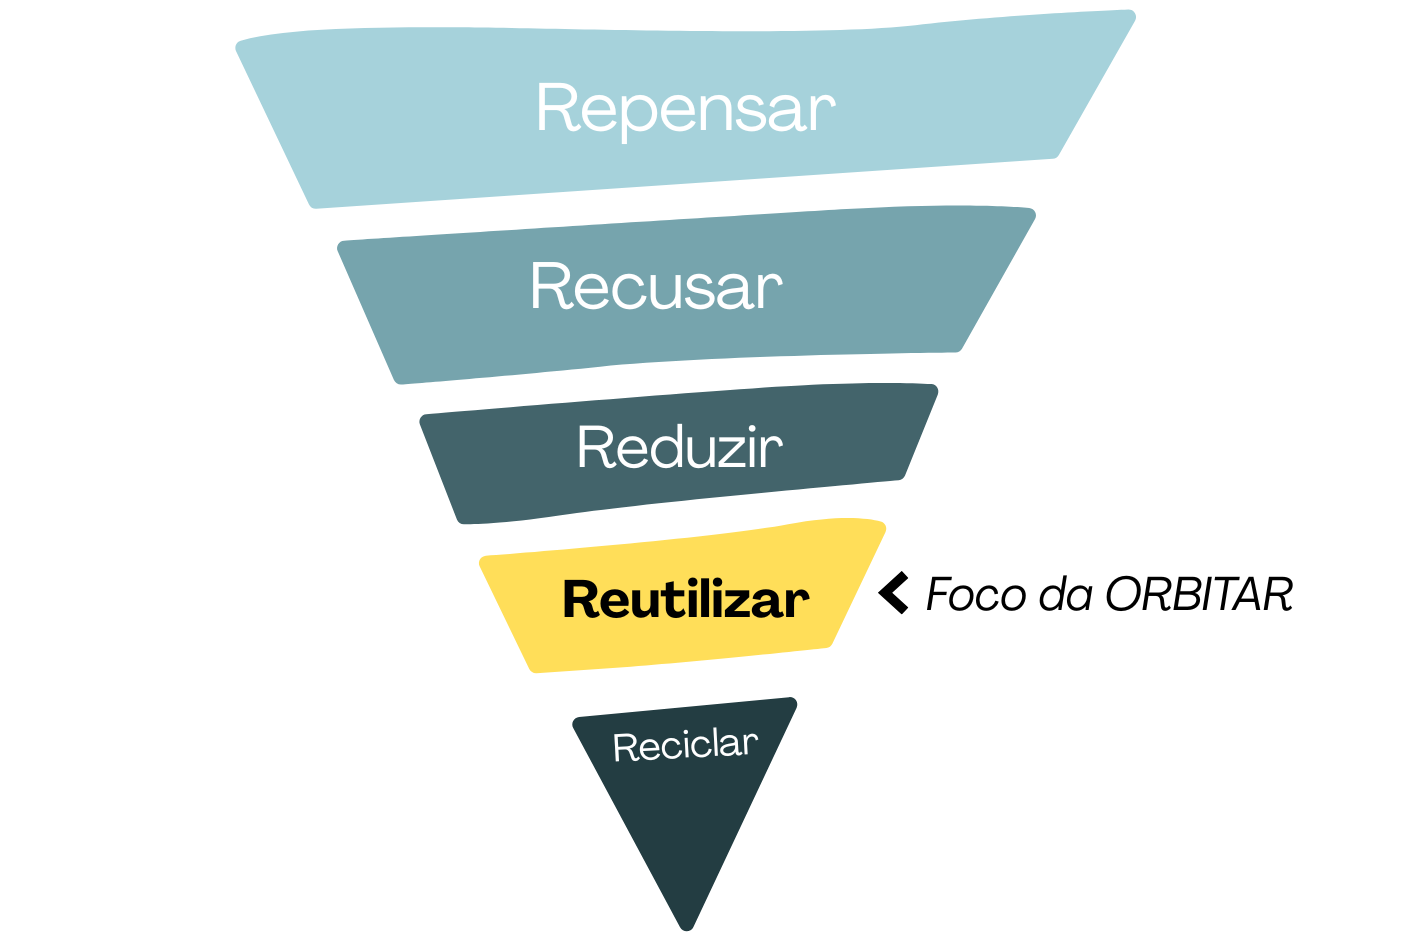
\includegraphics[width=0.7\textwidth]{imagens/hierarquia_5Rs.png}
    \caption{Hierarquia dos 5 Rs na Economia Circular.}
    \label{fig:hierarquia-5Rs}
    \legend{Fonte: Adaptado de Ellen MacArthur Foundation (2013), com destaque para a estratégia de Reutilização pela Orbitar.}
\end{figure}

O quadro a seguir (Quadro~\ref{quadro:linear-vs-circular}) sintetiza as principais diferenças entre os dois modelos econômicos.

\begin{quadro}[H] % <-- NOTA: [H] força o quadro a aparecer aqui.
    \caption{Comparativo entre Economia Linear e Economia Circular.}
    \label{quadro:linear-vs-circular}
    \begin{tabularx}{\textwidth}{lXX}
        \toprule % Linha superior do pacote booktabs
        \textbf{Critério} & \textbf{Economia Linear} & \textbf{Economia Circular} \\
        \midrule % Linha do meio do pacote booktabs
        \textbf{Fluxo} & Unidirecional (extrair-usar-descartar). & Cíclico e regenerativo. \\
        \textbf{Mentalidade} & Focada no consumo e na posse do produto. & Focada no uso, no acesso e no serviço. \\
        \textbf{Resíduos} & Vistos como um subproduto inevitável a ser gerenciado. & Vistos como uma falha de design a ser eliminada. \\
        \textbf{Valor} & O valor é destruído no final da vida útil do produto. & O valor é mantido e recirculado pelo maior tempo possível. \\
        \textbf{Estratégia} & Eficiência na produção em massa e obsolescência. & Reutilização, reparo, remanufatura e reciclagem. \\
        \bottomrule % Linha inferior do pacote booktabs
    \end{tabularx}
    \legend{Fonte: Elaborado pelo autor (2025), com base em Ellen MacArthur Foundation (2013).}
\end{quadro}

\section{A Reutilização como Ponte para a Inclusão Digital}

A estratégia de interceptar o descarte precoce através da reutilização cria uma oportunidade única de gerar impacto social positivo. Enquanto dispositivos funcionais são subutilizados ou descartados, uma parcela significativa da população brasileira ainda enfrenta a exclusão digital. Dados da pesquisa TIC Domicílios mostram que a posse de um computador, ferramenta essencial para a educação e qualificação profissional, ainda é um privilégio das classes de maior renda~\cite{cgi2024}.

A plataforma \textbf{Orbitar} se posiciona como uma ponte (Figura~\ref{fig:ponte-orbitar}) que conecta esses dois problemas, transformando o que seria um passivo ambiental em um ativo social. Ao facilitar que um eletrônico funcional chegue a quem precisa, o projeto aplica na prática os princípios da economia circular para combater a desigualdade digital.

\begin{figure}[H] % <-- NOTA: [H] força a figura a aparecer aqui.
    \centering
    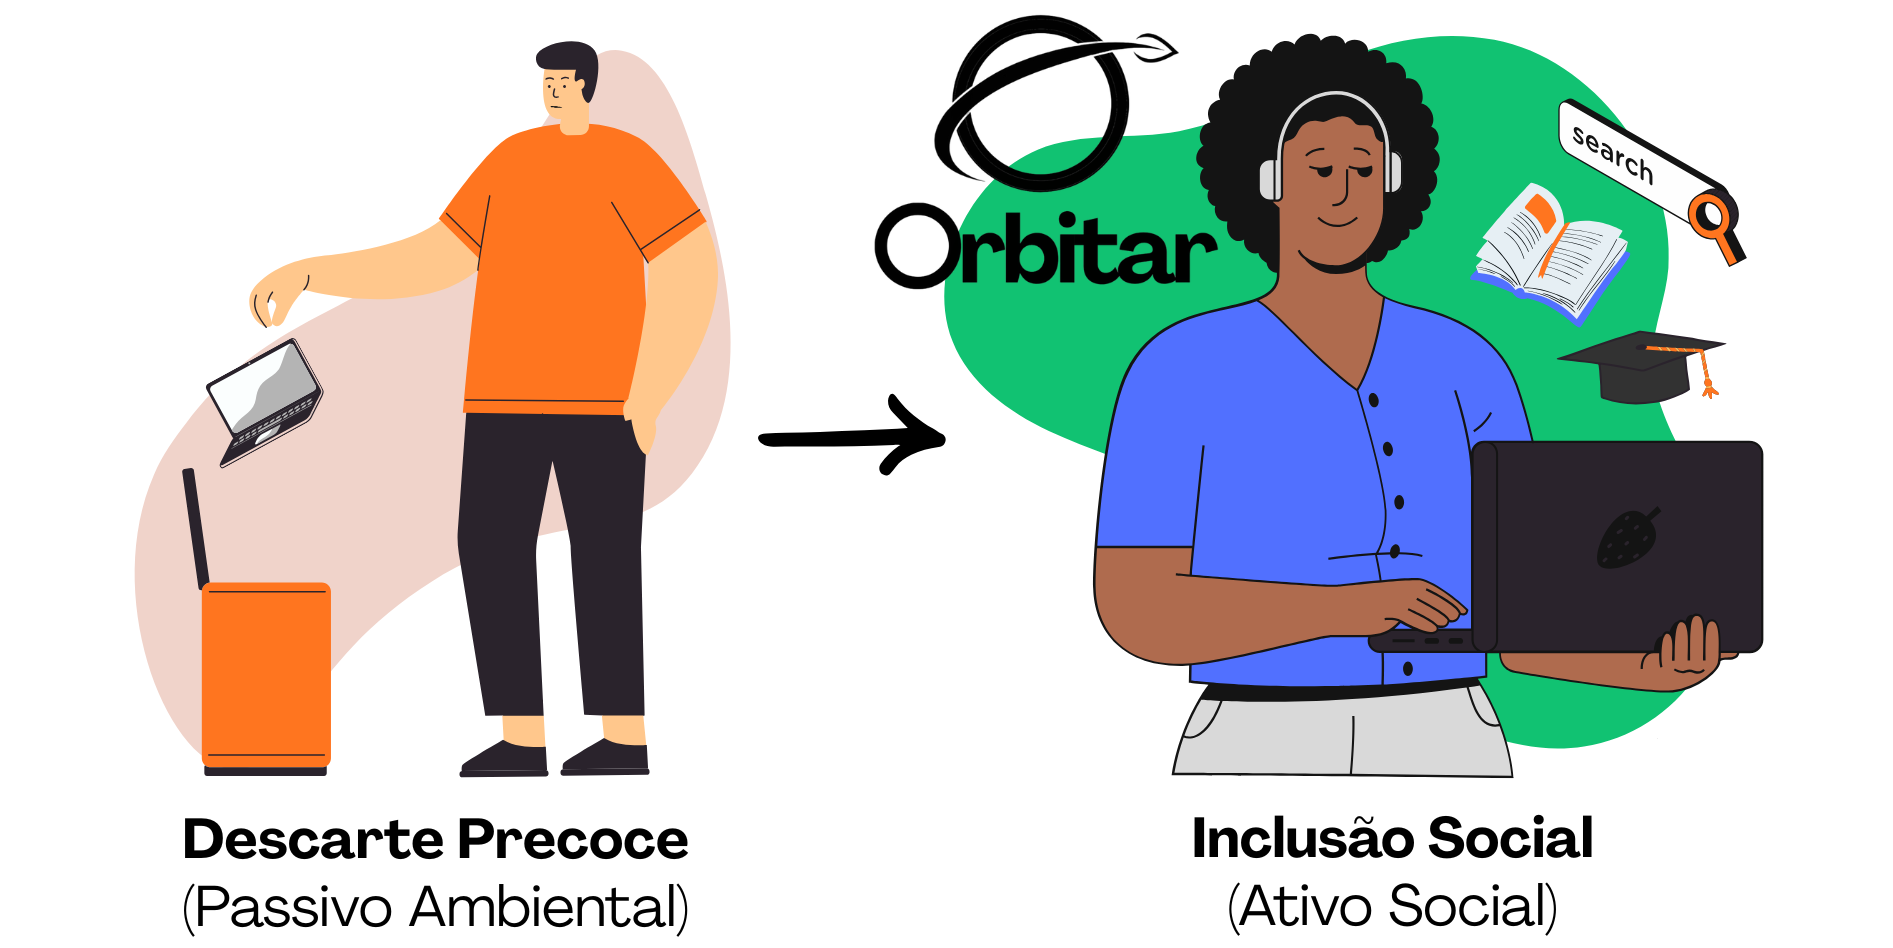
\includegraphics[width=0.7\textwidth]{imagens/compara.png}
    \caption{A Plataforma Orbitar como Ponte entre o Descarte Precoce e a Inclusão Digital.}
    \label{fig:ponte-orbitar}
    \legend{Fonte: Elaborado pelo autor (2025).}
\end{figure}


% =================================================================================
% CAPÍTULO 3 - REVISÃO DA LITERATURA
% =================================================================================
\chapter[Revisão Bibliográfica]{REVISÃO BIBLIOGRÁFICA}
Este capítulo apresenta uma análise do estado da arte de sistemas e plataformas voltados ao reaproveitamento de eletrônicos. A revisão visa identificar pesquisas e soluções existentes, suas contribuições e limitações e, consequentemente, as lacunas que o presente trabalho busca preencher.

\section{Procedimentos de Pesquisa e Análise Bibliográfica}

A pesquisa bibliográfica foi realizada em bases de dados científicas e repositórios relevantes, como Google Scholar, Scielo e ACM Digital Library, além da análise de plataformas comerciais e sociais consolidadas. As palavras-chave utilizadas, combinadas em diferentes configurações, foram:
\begin{itemize}
    \item "plataforma de doação de eletrônicos" ou "e-waste donation platform"
    \item "reutilização de lixo eletrônico" ou "e-waste reuse systems"
    \item "economia circular software" ou "circular economy platform"
    \item "inclusão digital e doação de computadores"
\end{itemize}
Foram selecionados trabalhos que descrevem a concepção ou análise de sistemas digitais, bem como plataformas já em operação, que servissem de base comparativa para a solução proposta.

\section{Soluções Nacionais para a Gestão de E-waste}

No Brasil, as iniciativas digitais de maior destaque para o descarte de e-waste focam majoritariamente na conexão do consumidor com pontos de reciclagem, em linha com a Política Nacional de Resíduos Sólidos.

A plataforma \textbf{E-cycle}~\cite{E-cycle} é um dos serviços mais conhecidos nesse segmento. Ela funciona como um robusto motor de busca que ajuda os usuários a encontrarem os postos de coleta mais próximos para uma vasta gama de resíduos, incluindo os eletrônicos. O seu mérito está em facilitar a logística reversa para a reciclagem. Contudo, sua abordagem não contempla a reutilização. A plataforma indica onde descartar um produto para que ele seja desmontado, mas não oferece uma via para que um equipamento funcional seja doado e continue em uso, o que representa uma lacuna em relação ao princípio de maior valor da economia circular.

No campo acadêmico, o trabalho de \cite{SilvaNeto2020} propôs o desenvolvimento de um aplicativo para gestão integrada de resíduos sólidos em uma cidade no Piauí, incluindo um módulo para doações. Embora a proposta seja relevante ao integrar a doação no fluxo de gestão de resíduos, sua principal limitação é a escala local e a ausência de um ecossistema focado na confiança e segurança necessárias para escalar uma rede de doações diretas entre usuários.

\section{Modelos e Soluções em Escala Global}

No cenário internacional, existem plataformas de grande escala que promovem o reaproveitamento de bens, servindo como referência para o modelo da \textbf{Orbitar}.

A \textbf{Freecycle Network}~\cite{Freecycle} é uma rede global sem fins lucrativos que promove a doação de itens para evitar que se tornem lixo. A plataforma opera por meio de grupos locais moderados por voluntários. Apesar do seu enorme sucesso e impacto positivo, seu modelo tecnológico, baseado em fóruns e listas de e-mail, apresenta barreiras de usabilidade para o usuário moderno, que espera uma experiência mais ágil, visual e geolocalizada, como a oferecida por aplicativos contemporâneos.

A iniciativa britânica \textbf{Donate a Tech}~\cite{DonateTech} tem um foco mais específico: a doação de equipamentos de TI (laptops, tablets) para instituições de caridade e escolas. A plataforma atua como uma intermediária, recebendo os equipamentos, realizando o recondicionamento e a limpeza de dados, e então os repassando. O modelo é muito eficaz para garantir a qualidade e a segurança dos dispositivos doados. No entanto, por ser \textbf{centralizado}, ele cria uma dependência logística da própria organização e não promove a conexão direta e ágil (peer-to-peer) entre o cidadão doador e o receptor final.

\section{Identificação de Lacunas e a Proposta Orbitar}

A análise dos trabalhos e plataformas existentes permitiu identificar as lacunas que justificam o desenvolvimento da \textbf{Orbitar}. O presente projeto se diferencia e contribui para a área ao:

\begin{itemize}
    \item \textbf{Integrar múltiplas fontes e focar na reutilização:} Diferente de sistemas como o E-cycle, que focam na reciclagem, a Orbitar prioriza a reutilização, a estratégia de maior valor agregado na economia circular.
    \item \textbf{Oferecer uma experiência de usuário moderna e descentralizada:} Em contraste com modelos como o da Freecycle ou da Donate a Tech, a Orbitar propõe uma plataforma web moderna, com interface intuitiva, geolocalização e um modelo peer-to-peer, que confere agilidade e escalabilidade à rede de doações.
    \item \textbf{Conectar as agendas ambiental e social de forma explícita:} A plataforma não se posiciona apenas como um meio de descarte correto, mas como uma ferramenta ativa de inclusão digital, dando visibilidade e propósito social ao ato da doação.
\end{itemize}

Dessa forma, este trabalho não apenas se apoia nos conhecimentos existentes, mas também busca oferecer uma solução inovadora, preenchendo a lacuna de uma plataforma nacional, descentralizada e focada em transformar o passivo do e-waste em um ativo para a inclusão social no Brasil.

\chapter[METODOLOGIA E DESENVOLVIMENTO]{METODOLOGIA E DESENVOLVIMENTO}

Escreva aqui a metodologia adotada no seu trabalho.

\chapter{Conclusão}

Escreva a sua conclusão do seu trabalho.


% ----------------------------------------------------------
% ELEMENTOS PÓS-TEXTUAIS
% ----------------------------------------------------------
\postextual{}

% ----------------------------------------------------------
% Referências bibliográficas
% ----------------------------------------------------------
\nocite{angular2024, dotnet2024, sqlserver2024}
\bibliographystyle{abntex2-alf}
\bibliography{bibliografia}  

% ----------------------------------------------------------
% Apêndices
% ----------------------------------------------------------
\begin{apendicesenv}
\partapendices{}
\chapter{Exemplo de Apêndice}
\end{apendicesenv}

% ----------------------------------------------------------
% Anexos
% ----------------------------------------------------------
\begin{anexosenv}
\partanexos{}
\chapter{Exemplo de Anexo}
\end{anexosenv}

\end{document}